
%(BEGIN_QUESTION)
% Copyright 2011, Tony R. Kuphaldt, released under the Creative Commons Attribution License (v 1.0)
% This means you may do almost anything with this work of mine, so long as you give me proper credit

Sketch wires in this diagram to show how a PLC could be connected to a Low-Pressure switch (PSL), a High-Pressure switch (PSH), and a motor contactor to control the starting and stopping of a three-phase air compressor motor, based on the ladder diagram PLC program shown in the computer display.  Note that several wires have already been properly connected for you:  

$$\includegraphics[width=15.5cm]{i02140x01.eps}$$

\underbar{file i02140}
%(END_QUESTION)





%(BEGIN_ANSWER)

{\it Award 4 points for each proper pressure switch connection, and 2 points for the proper contactor connection:}

$$\includegraphics[width=15.5cm]{i02140x02.eps}$$

\begin{itemize}
\item{} PSL Normally-Closed (NC) to X1 input
\item{} PSH Normally-Open (NO) to X2 input
\item{} Y3 output to contactor terminal A1
\end{itemize}

%(END_ANSWER)





%(BEGIN_NOTES)

{\bf This question is intended for exams only and not worksheets!}.

%(END_NOTES)


